\documentclass[twoside]{article}%{combine}
%\usepackage{url}
\usepackage{../../tex/html}
\usepackage{epstopdf}
\usepackage{amsfonts,amsmath,color,amsthm,amssymb, enumerate, bbm, subfig}
\usepackage{graphicx}
%\usepackage[DIV=14,BCOR=2mm,headinclude=true,footinclude=false]{typearea}
%\usepackage[font=small,labelfont=bf]{caption}
\usepackage{hyperref}
\usepackage{tikz, etoolbox}

\usetikzlibrary{shapes}
\usetikzlibrary{arrows}
%\usepackage[margin=1in]{geometry}
\usepackage{graphicx,amsmath,gentium,tikz,caption}
\usetikzlibrary{patterns}
\usetikzlibrary{matrix,arrows,positioning,shapes}
\usetikzlibrary{arrows.meta}
\tikzset{
  a/.style={-{Stealth[scale=1.3,angle'=45]},semithick}
}
%\usepackage{xfrac,fontspec,unicode-math}
%\setmathfont[version=cambria]{Cambria Math}
%\mathversion{cambria}
\usepackage[letterpaper, portrait, margin=1.1in]{geometry}
\usepackage{amsmath,amsthm}
\usepackage{mathtools}
\newtheorem*{definition}{Definition}
\usepackage{tcolorbox}
\tcbset{colback=white,colframe=black}
\everymath{\displaystyle}

\makeatletter
\@ifundefined{namelength}{
\newlength{\namelength}
\settowidth{\namelength}{{\bf \Large Name: }}
\newlength{\namelinelength}
\setlength{\namelinelength}{\textwidth}
\addtolength{\namelinelength}{-\namelength}
}{}

\@ifundefined{vs}{
\newcommand*{\vs}[1]{\par
  \vspace*{#1\baselineskip}%
  \@afterindentfalse
  \@afterheading
}
}{}
\makeatother



\def\fancytitle#1#2#3{
      \centerline{\framebox{\framebox{ \parbox{.8\textwidth}{ \bf ENGRI 1101 \hfill
      Engineering Applications of OR \ \ \ \  Fall 2020 \hfill #3 #1 \\
\mbox{ }\hfill
      \hfill\mbox{ } \\[1mm] \mbox{ } \hfill{\Large \bf #2}\hfill
      \mbox{ }} }}}
      
\vs 2
}

\def\handout#1#2{\fancytitle{#1}{#2}{Handout}}
\def\review#1#2{\fancytitle{#1}{#2}{Review}}
\def\homework#1#2{\fancytitle{#1}{#2}{Homework}}
\def\exercises#1{\fancytitle{}{#1}{Exercises}}
\def\solution#1#2{\fancytitle{#1}{#2}{Solutions}}
\def\final#1#2{\fancytitle{#1}{#2}{Final}
      \noindent {\bf \Large Name:} \rule{\namelinelength}{0.5pt}
      \vspace*{\baselineskip}}
\def\prelim#1#2{\fancytitle{#1}{#2}{Prelim}
      \noindent {\bf \Large Name:} \rule{\namelinelength}{0.5pt}
      \vspace*{\baselineskip}}
\def\quiz#1#2{\fancytitle{#1}{#2}{Quiz}
      \noindent {\bf \Large Name:} \rule{\namelinelength}{0.5pt}
      \vspace*{\baselineskip}}
\def\lab#1#2{\fancytitle{#1}{#2}{Lab}
      \noindent {\bf \Large Name:} \rule{\namelinelength}{0.5pt}
      \vspace*{\baselineskip}}
\def\prelab#1#2{\fancytitle{#1}{#2}{Prelab}
      \noindent {\bf \Large Name:} \rule{\namelinelength}{0.5pt}
      \vspace*{\baselineskip}}

\raggedbottom

\begin{document}

\prelab{1}{The Traveling Salesman Problem}

\textbf{Objectives}
\begin{itemize}
\item   Introduce students to a real world problem solved by OR practitioners
\item   Demonstrate the use of heuristics to obtain good solutions to optimization
problems
\item  Give students an appreciation of the difficulty of solving
optimization problems exactly
\end{itemize}

\vspace{2pt}


\noindent
Optional Reading Assignment:

\begin{itemize}
\item
Read Handout 2 on the traveling salesman problem.
\end{itemize}

\noindent
Pre-Lab Exercise:

Consider the drawing on the other side of this page, which is called a 
{\it graph}.
The circles represent cities, and are called the {\it nodes} of 
the graph, and the lines connecting pairs of nodes are called {\it edges}.
To determine the distance between a pair of points, one simply considers
the sum of the vertical distance and the horizontal between the two
nodes, where the length of each edge is 1. For example, the 
distance between the nodes labeled A and W
is 7 (3 vertical + 4 horizontal). Another way to view this distance
is the minimum number of edges that one must cross to get from one
point to the other.
For the traveling salesman problem, an ordering of cities is often
called a {\it tour}. 
\begin{enumerate}
\item   Find as good a tour as you can, and plot it on the graph itself .

\medskip
\item   How long is your tour?

\medskip
\item   What difficulties did you encounter in choosing your tour?
 
\medskip
\item   What methods did you use in finding this tour? 
Did you just eyeball it or did
you try to develop and apply a simple algorithm? Once you had a feasible
tour, did you try to improve upon it by changing it a little at a time or 
did you start again from scratch to try to find a better route?
\medskip
\item Can you give an explanation why this is the shortest tour?
(If you can prove that this is a shortest tour, then it is said
to be an {\it optimal} tour.)
\bigskip
\item Suppose that you considered a similar data set, but one in
which there were 7 rows and 7 columns of nodes (as opposed to 8 and 6
above, respectively). Can you find an optimal solution now?
How do you know that it is optimal? (This last question is not so easy.)
\end{enumerate}
\begin{figure}
\begin{center}
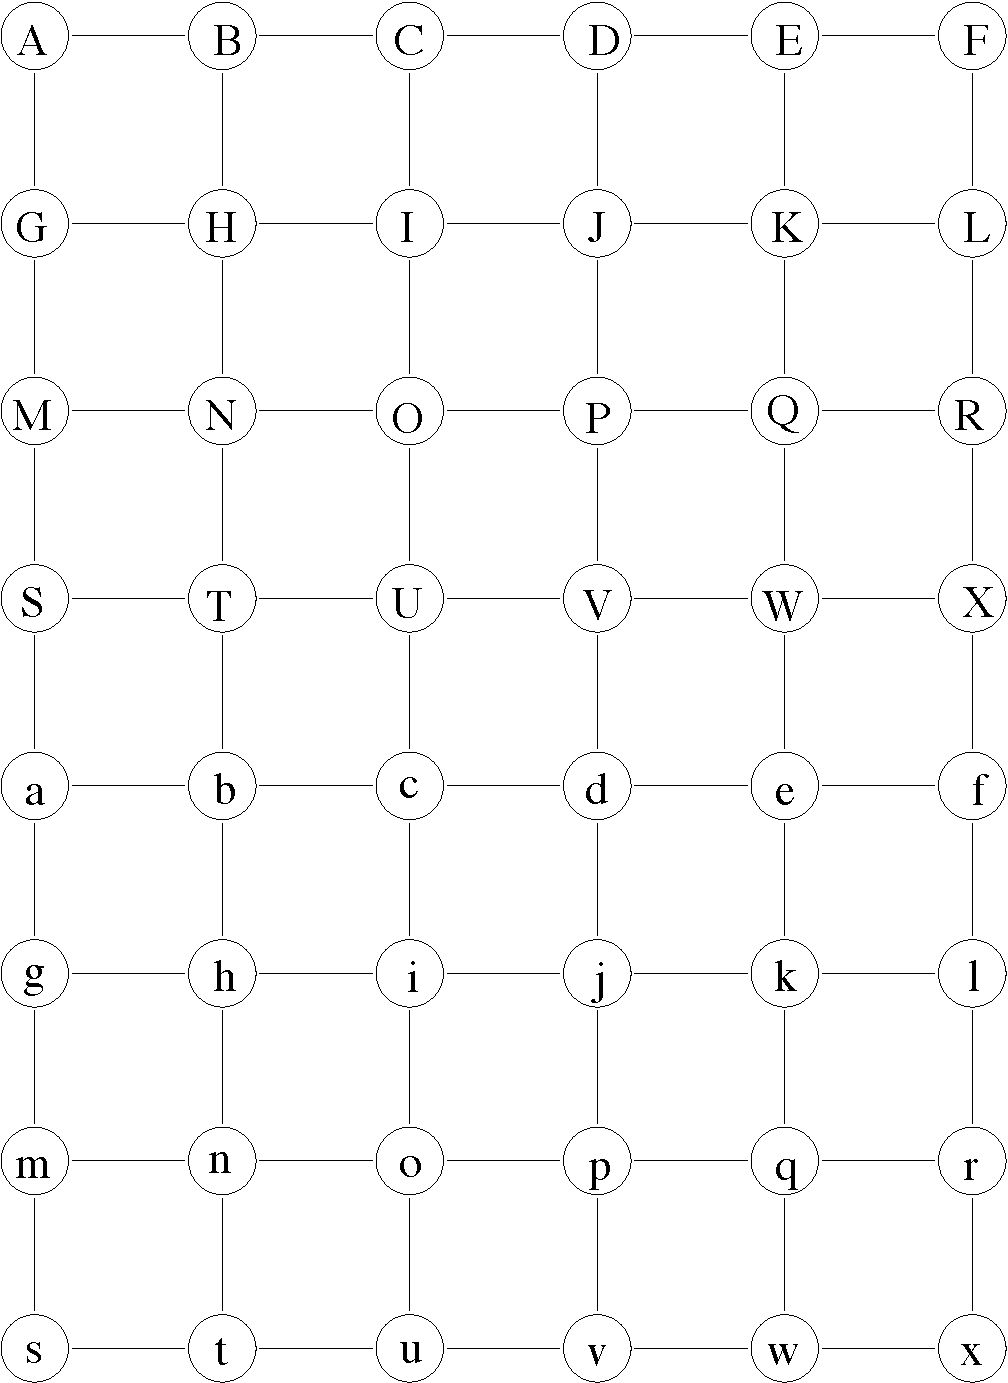
\includegraphics[height=10cm]{grid68.pdf}
\end{center}\end{figure}


\end{document} 
